\documentclass[../report.tex]{subfiles}
\begin{document}
\graphicspath{{img/}{../img/}}

\section{Vandfaldsmodellen \textsc{\textcolor{light-gray}{ - Nicki}}}

\label{sec:Vandfaldsmodellen}

Vandfaldsmodellen er en procesmodel, hvor man besk�ftiger sig med forskellige faser, en ad gangen, indtil man er n�et til slutningen af projektforl�bet. Denne model er ogs� kendt som one-shot eller once-through modellen, p� grund af dens ikke-iterative workflow. Modellen findes i forskellige udgaver, men den indeholder ofte disse fem faser; \textit{Kravspecifikation}, \textit{Design}, \textit{Implementering}, \textit{Verificering} og \textit{Vedligeholdelse}.  

\begin{figure}[H]
\centering
	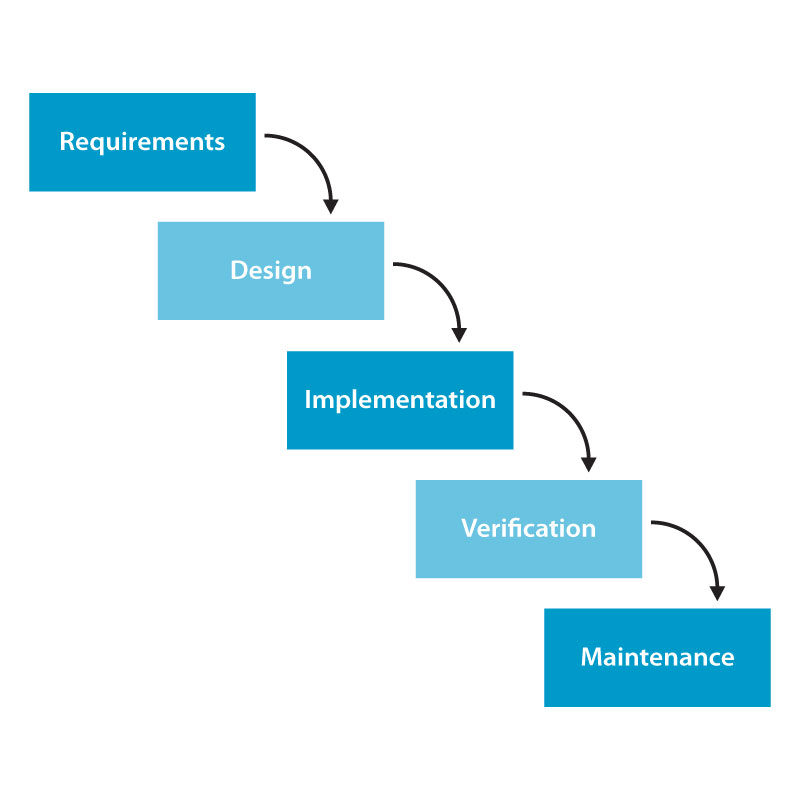
\includegraphics[scale=0.3]{h4_waterfall.jpg}
\caption{Vandfaldsmodellen med dens fem typiske faser}
\end{figure}

Retningen hvormed man arbejder med faserne skal altid v�re fremadg�ende eller nedadg�ende set i forhold til modellens analogi. Det er dog tilladt at ``plaske'' sig tilbage til den forrige fase, selvom dette er en undtagelse \cite[s 82]{hughescotterell09}.

\subsection{Styrker \& Svagheder}
Det stringente workflow som denne model indeholder giver begr�nsede muligheder for at iterere undervejs i projektet. Dette kan v�re en klar fordel, hvis kriterierne for projektet er veldefinerede og fastlagte fra start. Det er nemt at f�lge projektets udvikling undervejs b�de for udviklere, projektledere og for klienten, da hver fase naturligt genererer en milep�l for projektet. Dette betyder ogs� at det er nemt at evaluere p� den nyligt afsluttede fase, samt at estimere hvor meget der pr�cist mangler, f�r at projektet kan afsluttes \cite[s 83]{hughescotterell09}. \\

Vandfaldsmodellen er, som sagt, at foretr�kke hvis kriterierne for projektet er veldefinerede fra begyndelsen, og man er sikker p� at der ikke tilf�jes flere krav undervejs i processen. P� grund af den ikke-iterative arbejdsgang, er det ikke muligt at efterkomme nye krav undervejs. Modellen er generelt ufleksibel, da hver fase er fastlagt p� forh�nd. \\

En anden ulempe ved modellen er integrationen af produktet og muligheden for at klienten kan pr�ve produktet undervejs i forl�bet. F�rst efter implementerings-fasen vil man kunne fremvise et produkt til klienten, som derefter kan verificiere om det lever op til hans behov eller krav. \\

\subsection{Vandfaldsmodellen anvendt i target-projektet}

Hvis man i target-projektet havde valgt at arbejde stringent efter vandfaldmodellen, ville target-projektgruppen have v�ret n�dt til tydeligt at definere alle krav s� tidligt som muligt. Dette ville medf�re at man ville lukke for tilgangen af nye krav undervejs i projektet og ydermere betyde, at man ville have en tydelig definition af, hvilken funktionalitet der skulle implementeres, for at projektet kunne verificeres og afsluttes. \\

Dette ville have p�virket samarbejdet med de studerende fra Singapore. De singaporeanske studerendes opgave var at udvikle et system, der skulle samarbejde med det system der blev udviklet i target-projektet. Det bet�d at de kunne stille krav til dele af target-projektgruppens system. Dette ville have givet problemer, hvis de singaporeanske studerende gerne ville �ndre deres krav, efter kravspecifikationsfasen var overst�et. \\

Efterf�lgende faser som design- og implementationsfasen ville v�re tydeligt adskildte. I designfasen ville target-projektgruppen fokusere p� at definere interfaces, og p� at designe den overordnede systemarkitektur. Der ville slet ikke blive skrevet noget kode i denne fase. Til geng�ld ville der v�re meget fokus p� at dokumentere alle designbeslutningerne. \\

Implementeringsfasen ville best� i, at implementere alt koden til de interfaces, der var blevet defineret i designfasen. Dette burde v�re en nem opgave, da systemets design ville v�re tydeligt defineret og dokumenteret inden p�begyndelsen af implementeringen. Target-projektgruppen skulle dog helst undg� at ``plaske'' sig tilbage til en tidligere fase. Noget de kunne blive fristet til, hvis de singaporeanske studerende pressede p� for at f� indf�rt nogle nye krav til systemet, som det ikke var designet til at h�ndtere i designfasen.

\end{document}